\documentclass{beamer}
\usepackage[latin1]{inputenc}
\usepackage{xcolor}
\usepackage{hyperref}
\usepackage{minted}
\usepackage{graphicx}
\usepackage{tikz}
\usetikzlibrary{fadings,tikzmark,calc,positioning,decorations.pathreplacing}
\usepackage{bm}
\usepackage{bbding} % For \HandRight
\usepackage{fancyvrb} % For \UseVerb \SaveVerb
\usepackage{mathtools} % For aligning matrix columns

\usetheme{Madrid}
\usecolortheme{default}

% Command that embeds a hand pointing to the right in a href label
\newcommand{\hrefhand}[2]{\raisebox{-0.4ex}{\HandRight}\,\href{#1}{#2}}

\title{COMP3320 Introduction to OpenGL}
\author{Alex Biddulph}
\institute{
    The University of Newcastle, Australia
    \and
    Based on the work provided at \url{www.learnopengl.com}
}
\date{Semester 2, 2021}

\begin{document}

\begin{frame}
    \titlepage
\end{frame}

\begin{frame}[fragile]{Object Colour}
    \begin{itemize}
        \item The colour that an object reflects
        \item This can be simulated as a simple multiplication
              \footnotesize{
                  \begin{minted}{glsl}
    vec3 light_colour  = vec3(1.0f, 1.0f, 1.0f);
    vec3 object_colour = vec3(1.0f, 0.5f, 0.31f);
    // This is a component-wise multiplication
    vec3 result        = light_colour * object_colour;
\end{minted}
              }
    \end{itemize}

    \begin{figure}
        \centering
        \includegraphics[height=0.30\textheight]{images/light_reflection.png}
        \caption{\footnotesize{Image sourced from \url{learnopengl.com/Lighting/Colors}}}
    \end{figure}
\end{frame}

\begin{frame}[fragile]{Basic Lighting}
    \begin{figure}
        \centering
        \includegraphics[height=0.30\textheight]{images/basic_lighting_phong.png}
        \includegraphics[height=0.30\textheight]{images/basic_lighting_gouruad.png}
        \caption{\footnotesize{Images sourced from \url{learnopengl.com/Lighting/Basic-Lighting}}}
    \end{figure}
\end{frame}

\begin{frame}[fragile]{Basic Lighting}
    \begin{itemize}
        \item Ambient: Background/global lighting. Results in objects being dimly lit when all
              other lights are turned off.
        \item Diffuse: Brightness of reflected light is dictated by how closely the fragments
              normal vector aligns with the light direction.
        \item Specular: Light is reflected about the fragments normal vector. Light appears
              brightest when the viewing direction most closely aligns with the reflected direction.
    \end{itemize}

    \begin{figure}
        \includegraphics[height=0.30\textheight]{images/diffuse_light.png}
        \includegraphics[height=0.30\textheight]{images/specular_light.png}
        \caption{\footnotesize{Images sourced from \url{learnopengl.com/Lighting/Basic-Lighting}}}
    \end{figure}
\end{frame}

\begin{frame}[fragile]{Basic Lighting Equations}
    \begin{itemize}
        \item Ambient:
              \footnotesize{
                  \begin{minted}{glsl}
vec3 ambient = ambient_strength * light_colour;
vec3 result  = ambient * object_colour;
\end{minted}
              }
        \item Diffuse:
              \footnotesize{
                  \begin{minted}{glsl}
vec3 norm           = normalize(frag_normal);
vec3 light_dir      = normalize(light_pos - frag_pos);
float diff_strength = max(dot(norm, light_dir), 0.0f);
vec3 diffuse        = diff_strength * light_colour;
vec3 result         = diffuse * object_colour;
\end{minted}
              }
    \end{itemize}
\end{frame}

\begin{frame}[fragile]{A Couple of Notes}
    \begin{block}{A Note on Content}
        The next slide contains a reference to homogeneous transformations, rotations, and matrices. If you don't know what these are or need a refresher be sure to check the Transformations lecture.
    \end{block}

    \begin{block}{A Note on Notation}
        The next slide uses a different notation for homogeneous transformations that is not used in the Transformations lecture. If you would like more information on this notational style see \hrefhand{https://nubook.nubots.net/system/foundations/mathematics\#homogeneous-transformations}{NUbook}
    \end{block}
\end{frame}

\begin{frame}[fragile]{Non-Uniform Object Scaling}
    \begin{itemize}
        \item If objects are not scaled uniformly then normals can point in strange directions
        \item To account for this use the inverse transpose of the model-view rotation matrix
        \item If $H^{v}_{m}$ is a homogeneous transformation matrix that transforms vectors from model space to view space, then $R^{v}_{m}$ is the top-left 3x3 corner of the model-view matrix and forms the rotation component of the transformation
              $$
                  H^{v}_{m} = \begin{bmatrix}
                      \bm{R}^{v}_{m}     & \bm{\vec{r}}^{v}_{MV} \\
                      \bm{\vec{0}}_{1x3} & 1
                  \end{bmatrix}
              $$
        \item To account for non-uniform object scaling we can multiply our vertex normals by
              $$\bm{N}^{v}_{m} = \left(\left(\bm{R}^{v}_{m}\right)^{'}\right)^{T}$$
        \item This is the inverse transpose of $\bm{R}^{v}_{m}$ and is known as \hrefhand{http://www.lighthouse3d.com/tutorials/glsl-12-tutorial/the-normal-matrix/}{\color{blue}the normal matrix}
    \end{itemize}
\end{frame}

\begin{frame}[fragile]{Basic Lighting Equations}
    \begin{itemize}
        \item Specular:
              \footnotesize{
                  \begin{minted}{glsl}
vec3  norm        = normalize(frag_normal);
vec3  light_dir   = normalize(frag_pos - light_pos);
vec3  view_dir    = normalize(view_pos - frag_pos);
vec3  reflect_dir = reflect(light_dir, norm);
float strength    = pow(max(dot(view_dir, reflect_dir), 0.0f), 32.0f);
vec3  specular    = 0.5f * strength * light_colour;
vec3  result      = specular * object_colour;
\end{minted}
              }
    \end{itemize}

    \SaveVerb{strength}|strength|
    \begin{figure}
        \centering
        \includegraphics[height=0.30\textheight]{images/specular_shininess.png}
        \caption{The effect of {\color{blue}\UseVerb{strength}} (the shininess factor) on the specular highlight. \footnotesize{Images sourced from \url{learnopengl.com/Lighting/Basic-Lighting}}}
    \end{figure}

    \begin{tikzpicture}[remember picture, overlay]
        \node[rectangle,minimum width=0.95cm,minimum height=0.35cm,draw=red,ultra thick] at (11.65cm, 5.80cm) (P) {};
        \draw[ultra thick,red,<-] (P.south) -- (11.00cm, 5.00cm) node[anchor=north] {Shininess};
    \end{tikzpicture}
\end{frame}

\begin{frame}[fragile]{Lighting Maps}
    \begin{itemize}
        \item Use textures to provide object colour per fragment.
        \item Use textures to specify which areas of an object give specular reflections
              \begin{center}
                  \includegraphics[height=0.30\textheight]{images/container_diffuse.png}
                  \includegraphics[height=0.30\textheight]{images/container_specular.png}
              \end{center}
        \item Use a single uniform to provide material properties per object
              \footnotesize{
                  \begin{minted}{glsl}
    struct Material {
        sampler2D diffuse;
        sampler2D specular;
        float shininess;
    };
    in vec2 texture_coordinates;
    uniform Material material;
\end{minted}
              }
        \item Use the equations as before, but sample the appropriate texture to get {\color{blue}\verb"object_colour"}.
    \end{itemize}
    \vfill{}
    {\footnotesize{Images sourced from \url{learnopengl.com/Lighting/Basic-Lighting}}}
\end{frame}

\begin{frame}[fragile]{Types of Light}
    \begin{itemize}
        \item Directional: Light source is very far away. When the light reaches the object
              light rays are basically parallel to each other.
        \item Point Light: A nearby light that illuminates equally in all directions.
        \item Spot Light: A nearby light that illuminates in a single direction.
    \end{itemize}
\end{frame}

\begin{frame}[fragile]{Light Attenuation}
    \begin{itemize}
        \item Light intensity drops off over distance
        \item A common formula for attentuation is
              $$F_{att} = \frac{1}{K_{c} + K_{l}d + K_{q}d^{2}}$$
        \item $K_{c}$ represents a constant amount of attentuation regardless of listance
        \item $K_{d}$ represents a attentuation that is linearly proportional to distance
        \item $K_{q}$ represents a attentuation that is quadratically proportional to distance
        \item Use trial and error to find some good values or use some \hrefhand{https://wiki.ogre3d.org/tiki-index.php?page=-Point+Light+Attenuation}{\color{blue}pre-calculated values}
    \end{itemize}
\end{frame}

\begin{frame}[fragile]{Spotlight Smoothing}
    \begin{itemize}
        \item Represent spotlight as a cone
        \item If light stops at edge of cone there will be a hard line between light/no light
        \item Instead represent spotlight with two cones and fade spotlight intensity between them
        \item $\theta$ is the angle between the spotlight direction and the fragment position
        \item $\phi$ and $\gamma$ are the angles between the spotlight direction and the inner and outer cones
    \end{itemize}

    \begin{figure}
        \centering
        \scalebox{1.00}{
            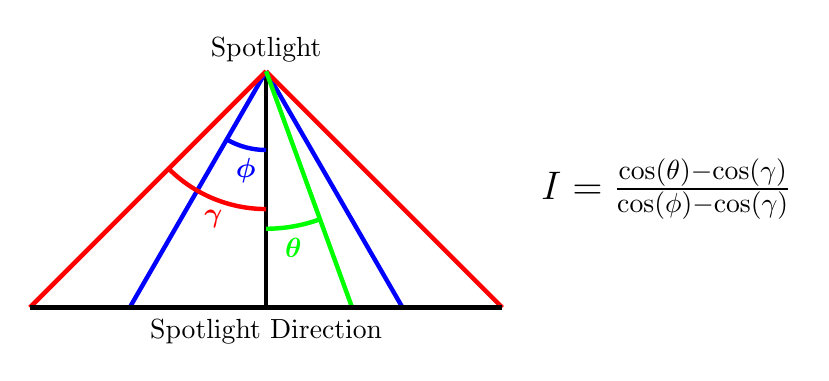
\begin{tikzpicture}
                \node[above] at (0.00cm, 0.00cm) (L) {Spotlight};
                \draw[ultra thick] (0.00cm, 0.00cm) -- (0.00cm, -3.00cm) node[below] {Spotlight Direction};
                \draw[ultra thick,blue] (0.00cm, 0.00cm) -- (-1.732cm, -3.00cm);
                \draw[ultra thick,red] (0.00cm, 0.00cm) -- (-3.00cm, -3.00cm);
                \draw[ultra thick,blue] (0.00cm, 0.00cm) -- (1.732cm, -3.00cm);
                \draw[ultra thick,red] (0.00cm, 0.00cm) -- (3.00cm, -3.00cm);
                \draw[ultra thick,green] (0.00cm, 0.00cm) -- (1.092cm, -3.00cm);
                \draw[ultra thick] (-3.00cm, -3.00cm) -- (3.00cm, -3.00cm);
                \draw[ultra thick,blue] (0.00cm, -1.00cm) arc (270:240:1.00cm) node[midway,below]{$\bm{\phi}$};
                \draw[ultra thick,red] (0.00cm, -1.75cm) arc (270:225:1.75cm) node[midway,below]{$\bm{\gamma}$};
                \draw[ultra thick,green] (0.00cm, -2.00cm) arc (270:290:2.00cm) node[midway,below]{$\bm{\theta}$};

                \node at (5.00cm, -1.5cm) {
                    \Large{
                        $I = \frac{\cos\left(\theta\right) - \cos\left(\gamma\right)}{\cos\left(\phi\right) - \cos\left(\gamma\right)}$}
                };
            \end{tikzpicture}
        }
    \end{figure}
\end{frame}

\begin{frame}[fragile]{Types of Light}
    \begin{itemize}
        \item Directional:
              \footnotesize{
                  \begin{minted}{glsl}
    struct DirectionalLight {
        vec3 direction;

        vec3 ambient;
        vec3 diffuse;
        vec3 specular;
    };
    uniform DirectionalLight sun;
\end{minted}
              }
        \item Point Light:
              \footnotesize{
                  \begin{minted}{glsl}
    struct PointLight {
        vec3 position;

        vec3 ambient;
        vec3 diffuse;
        vec3 specular;

        float Kc;
        float Kl;
        float Kq;
    };
    uniform PointLight ceiling_light;
\end{minted}
              }
    \end{itemize}
\end{frame}

\begin{frame}[fragile]{Types of Light}
    \begin{itemize}
        \item Spot Light:
              \footnotesize{
                  \begin{minted}{glsl}
    struct SpotLight {
        vec3 position;
        vec3 direction;

        vec3 ambient;
        vec3 diffuse;
        vec3 specular;

        float Kc;
        float Kl;
        float Kq;

        float phi;
        float gamma;
    };
    uniform SpotLight torch;
\end{minted}
              }
    \end{itemize}
\end{frame}

\end{document}
